%!TEX root=cvFioretto.tex
%Section: Scholarships and additional info
\sectionTitle{Publications}{}%{\faBook}

\begin{keywords}
\keywordsentry{\textbf{Summary}:}
{			 \faAngleRight~ \nemph{13} Journals articles
\hspace{4pt} \faAngleRight~ \nemph{60} Conference papers
\hspace{4pt} \faAngleRight~ \nemph{2} Book chapters
\hspace{4pt} \faAngleRight~ \nemph{3} Editorial articles
\hspace{4pt} \faAngleRight~ \nemph{19} Workshop papers
\hspace{4pt} \faAngleRight~ \nemph{20+} Preprints
}
\keywordsentry{\textbf{Total citations}:}
{\citNo \hspace{8pt} 
 \textbf{H-index}: \hIndex \hspace{8pt} 
 \gscholar{Google Scholar} 
 %\textbf{CS-rankings [from 2019]:} \nemph{12} (count)
 }% \faExternalLink}} 
\end{keywords}
%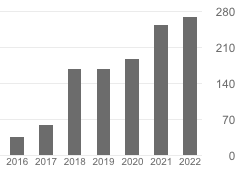
\includegraphics[height=30pt]{scholar-cit.png}

Names of students I supervise(d) are prepended with symbol \student{}.


\iffalse
\subsectionTitle{Under review}

% 2024 %%%%%%%%%%%%%%%%%%%%%%%%%%%%%%%%%%%%%%%%%%%%%%%%%%%%%%%%%%%%%%%%%%%%%%%%%%%%%%%%%
\begin{pubs}

\wsentry
	{}
	{\student{} Cuong Tran, Zarreen Reza, {\bf Ferdinando Fioretto}}
  	{On the unintended fairness effects of Low Rank Approximation in Large Language Models}
	{\procACL, 2024}
	{}
	
\wsentry
	{}
	{\student{} Razane Tajeddine, Ajinkya Mulay, Tudor Cebere, {\bf Ferdinando Fioretto}}
  	{From Adversarial Robustness to Differential Privacy and Back}
	{\procUAI, 2024}
	{}

\wsentry
	{}
	{\student{} James Kotry, \student{} My H.~Dinh, {\bf Ferdinando Fioretto}}
  	{End-to-End Optimization and Learning with Ordered Weighted Averages}
	{\procUAI, 2024}
	{}

\wsentry
	{}
	{\student{} Jacob K Christopher, {\bf Ferdinando Fioretto}}
  	{Projected Generative Diffusion Models for Constraint Satisfaction}
	{\procICML, 2024}
	{}
\wsentry
	{}
	{Khang Tran, {\bf Ferdinando Fioretto}, Issa Khalil, My T. Thai, Linh Thi Xuan Phan, Hai Phan}
  	{Achieving Fairness Certification with Differential Privacy}
	{\procICML, 2024}
	{}

\wsentry
	{}
	{\student{} Saswat Das, Marco Romanelli, {\bf Ferdinando Fioretto}}
	{Disparate Impact on Group Accuracy of Linearization for Private Inference}
	{\procICML, 2024}
	{}

\wsentry
	{}
	{Sree Harsha Nelaturu, Nishaanth Kanna Ravichandran, \student{} Cuong Tran, Sara Hooker, {\bf Ferdinando Fioretto}}
	{On The Fairness Impacts of Hardware Selection in Machine Learning}
	{\procICML, 2024}
	{}

\wsentry
	{}
	{Prakhar Ganesh, \student{} Cuong Tran, Reza Shokri, {\bf Ferdinando Fioretto}}
	{The Data Minimization Principle in Machine Learning}
	{\procFAccT, 2024}
	{}

\wsentry
	{}
	{\student{} My H.~Dinh, \student{} James Kotary, {\bf Ferdinando Fioretto}}
	{Learning Fair Ranking Policies via Differentiable Optimization of Ordered Weighted Averages}
	{\procFAccT, 2024}
	{}

\wsentry
	{}
	{\student{} James Kotary, \student{} Vincenzo Di Vito, \student{} Jacob K Christopher, Pascal Van Hentenryck, {\bf Ferdinando Fioretto}}
	{Learning Joint Models of Prediction and Optimization}
	{\procIJCAI, 2024}
	{}

\wsentry
	{}
	{\student{Cuong Tran}, Keyu Zhu, {\bf Ferdinando Fioretto}, Pascal Van Hentenryck}
	{Fairness Increases Adversarial Vulnerability}
	{\procIJCAI, 2024}
	{https://arxiv.org/abs/2211.11835}
\end{pubs}

\subsectionTitle{Refereed Conferences or Journal Papers}
\fi

\begin{pubs}
%{\nemph{Refereed Conferences or Journal Papers}}&\nemph{\rule{0.5\linewidth}{0.5pt}}\\[1em]
% 2024 %%%%%%%%%%%%%%%%%%%%%%%%%%%%%%%%%%%%%%%%%%%%%%%%%%%%%%%%%%%%%%%%%%%%%%%%%%%%%%%%%
% {\nemph{2020}}&\nemph{\rule{0.5\linewidth}{0.5pt}}\\[1em]

\wsentry
	{124}
	{\student{} James Kotary, {\bf Ferdinando Fioretto}}
	{Learning Constrained Optimization with Deep Augmented Lagrangian Methods}
	{\venue{CoRR abs}/2403.03454, 2024}
	{https://arxiv.org/abs/2403.03454}

\wsentry
	{123}
	{\student{}My H. Dinh, \student{} James Kotary, {\bf Ferdinando Fioretto}}
	{End-to-End Learning for Fair Multiobjective Optimization Under Uncertainty}
	{\venue{CoRR abs}/2402.07772, 2024}
	{https://arxiv.org/abs/2402.07772}

\wsentry
	{122}
	{\student{} Jacob K Christopher, {\bf Ferdinando Fioretto}}
  	{Projected Generative Diffusion Models for Constraint Satisfaction}
	{\venue{CoRR abs}/2402.03559, 2024}
	{https://arxiv.org/abs/2402.03559}

\wsentry
	{121}
	{\student{} Saswat Das, Marco Romanelli, {\bf Ferdinando Fioretto}}
	{Disparate Impact on Group Accuracy of Linearization for Private Inference}
	{\venue{CoRR abs}/2402.03629, 2024}
	{https://arxiv.org/abs/2402.03629}

\wsentry
	{120}
	{\student{} My H.~Dinh, \student{} James Kotary, {\bf Ferdinando Fioretto}}
	{Learning Fair Ranking Policies via Differentiable Optimization of Ordered Weighted Averages}
	{\venue{CoRR abs}/2402.05252, 2024}
	{https://arxiv.org/abs/2402.05252}

\confentry
	{119}
	{{\bf Ferdinando Fioretto}, Keyu Zhu, Pascal Van Hentenryck, \student{} Saswat Das and Christine Task}
  	{Finding $\epsilon$ and $\delta$ of Traditional Disclosure Control Systems}
	{\procAAAI, 2024}
	{https://arxiv.org/abs/2301.12204}
	{23.75\%}

\wsentry
	{118}
	{\student{James Kotary}, \student{Jacob Christopher}, \student{My H Dinh},
	and {\bf Ferdinando Fioretto}}
	{Analyzing and Enhancing the Backward-Pass Convergence of Unrolled Optimization}	
	{\venue{CoRR abs}/2301.12047, 2024}
	{https://arxiv.org/abs/2301.12047}


% 2023 %%%%%%%%%%%%%%%%%%%%%%%%%%%%%%%%%%%%%%%%%%%%%%%%%%%%%%%%%%%%%%%%%%%%%%%%%%%%%%%%%
% {\nemph{2020}}&\nemph{\rule{0.5\linewidth}{0.5pt}}\\[1em]
\wsentry
	{117}
	{\student{} Sree Harsha Nelaturu, \student{} Nishaanth Kanna Ravichandran, \student{} Cuong Tran, Sara Hooker, and {\bf Ferdinando Fioretto}}
	{On The Fairness Impacts of Hardware Selection in Machine Learning}	
	{\venue{CoRR abs}/2312.03886, 2023}
	{https://arxiv.org/abs/2312.03886}

\journalentry
	{116}
	{Mostafa Mohammadian, Kyri Baker, \textbf{Ferdinando Fioretto}}
	{Gradient-Enhanced Physics-Informed Neural Networks for Power Systems Operational Support}
	{Electric Power Systems Research, pages 109551, 2023}
	{https://www.sciencedirect.com/science/article/abs/pii/S0378779623004406}

\confentry
	{115}
	{\student{Cuong Tran} and {\bf Ferdinando Fioretto}}
	{Data Minimization at Inference Time}
	{\procNeurIPS, 2023}
	{https://arxiv.org/abs/2305.17593}
	{23\%}

\wsentry
	{114}
 	{Vladimir Dvorkin and {\bf Ferdinando Fioretto}}
  	{Price-Aware Deep Learning for Electricity Markets}
  	{Tackling Climate Change with Machine Learning, at NeurIPS 2023}
  	{https://arXiv.org/abs/2308.01436}

\confentry
	{113}
	{\student{My H. Dinh}, {\bf Ferdinando Fioretto}, Mostafa Mohammadian, and Kyri Baker}
	{An Analysis of the Reliability of AC Optimal Power Flow Deep Learning Proxies}
	{IEEE PES Innovative Smart Grid Technologies, 2023}
	{https://arxiv.org/abs/2111.11168}
	{unknown}

\confentry 
	{112} %{IJCAI}
	{\student{James Kotary}, \student{My H. Dinh}, {\bf Ferdinando Fioretto}}
	{Folded Optimization for End-to-End Model-Based Learning}
	{\procIJCAI, 2023}
	{https://arxiv.org/abs/2301.12047}
	{15\%}

\confentry
    {111} %{IJCAI}
	{\student{James Kotary}, \student{Vincenzo Di Vito}, {\bf Ferdinando Fioretto}, Pascal Van Hentenryck}
	{SF-PATE: Scalable, Fair, and Private Aggregation of Teacher Ensembles}
    {\procIJCAI, 2023}
	{https://arxiv.org/abs/2204.05157}
    {15\%}

\confentry
    {110} %{IJCAI}
	{\student{Cuong Tran}, \student{Keyu Zhu}, {\bf Ferdinando Fioretto}}
	{End-to-End Combinatorial Ensemble Learning}
    {\procIJCAI, 2023}
	{http://arxiv.org/abs/2211.00251}
    {15\%}

\confentry
    {109} %{IJCAI}
	{\student{Cuong Tran}, {\bf Ferdinando Fioretto}}
	{On the Fairness Impacts of Private Ensembles Models}
    {\procIJCAI, 2023}
	{http://arxiv.org/abs/2109.08630}
    {15\%}

\wsentry
	{108} %{PES}
	{Terrence W.K. Mak, {\bf Ferdinando Fioretto}, Pascal Van Hentenryck}
	{Load Encoding for Learning AC-OPF}
	{Proceedings of the \venue{IEEE PES General Meeting (PES)}, 2023}
	{https://arxiv.org/abs/2101.03973}

\confentry
    {107} %{AAMAS}
	{\student{James Kotary}, \student{Vincenzo Di Vito}, {\bf Ferdinando Fioretto}}
	{End-to-End Optimization and Learning for Multiagent Ensembles}
    {\procAAMAS, 2023}
	{http://arxiv.org/abs/2211.00251}
    {40\%}

\wsentry
	{106}
	{Jayanta Mandi, \student{James Kotary}, Senne Berden, Maxime Mulamba, Victor Bucarey, Tias Guns, {\bf Ferdinando Fioretto}} 
	{Decision-Focused Learning: Foundations, State of the Art, Benchmark and Future Opportunities}
	{\venue{CoRR abs}/2307.13565, 2023}
	{https://arxiv.org/abs/2307.13565}

\wsentry
	{105}
	{Khang Tran, {\bf Ferdinando Fioretto}, Issa Khalil, My T. Thai, NhatHai Phan} 
	{FairDP: Certified Fairness with Differential Privacy}
	{\venue{CoRR abs}/2305.16474, 2023}
	{https://arxiv.org/abs/2305.16474}

\wsentry 
	{104}%{ArXiv}
	{Keyu Zhu, {\bf Ferdinando Fioretto}, Pascal Van Hentenryck, Saswat Das, Christine Task}
	{Privacy and Bias Analysis of Disclosure Avoidance Systems}
	{\venue{CoRR abs}/2301.12204, 2023}
	{https://arxiv.org/abs/2301.12204}

\wsentry 
	{103}%{ArXiv}
	{\student{My H. Dinh}, {\bf Ferdinando Fioretto}}
	{Context-Aware Differential Privacy for Language Modeling}
	{\venue{CoRR abs}/2301.12288, 2023}
	{https://arxiv.org/abs/2301.12288}


% 2022 %%%%%%%%%%%%%%%%%%%%%%%%%%%%%%%%%%%%%%%%%%%%%%%%%%%%%%%%%%%%%%%%%%%%%%%%%%%%%%%%%

\journalentry
	{102} %{JAIR}
	{Khoi D.~Hoang, \textbf{Ferdinando Fioretto}, Ping Hou, William Yeoh, Makoto Yokoo, Roie Zivan}
	{Proactive Dynamic Distributed Constraint Optimization Problems}
	{\JAIR, (73), pages 179-225, 2022}
	{https://www.jair.org/index.php/jair/article/view/13499}
\confentryAwd
	{101} %{NeurIPS}
	{\student{Cuong Tran}, {\bf Ferdinando Fioretto}, Jung-Eun Kim, 
	\student{Rakshit Naidu}}
	{Pruning has a disparate impact on model accuracy}
	{\procNeurIPS, 2022}
	{http://arxiv.org/abs/2205.13574}
	{25.6\%} %48
	{Lightning Talk (Spotlight)}
	{(Typically assigned to $\sim$3\% out of all paper submissions (10,411, in 2022))}
\confentry
	{100} %{IJCAI}
	{Keyu Zhu, {\bf Ferdinando Fioretto}, Pascal Van Hentenryck}
	{Post-processing of Differentially Private Data: A Fairness Perspective}
	{\procIJCAI, 2022}
	{http://arxiv.org/abs/2202.09425}	
	{15\%}
\confentry
	{99} %{IJCAI}
	{{\bf Ferdinando Fioretto}, \student{Cuong Tran}, Keyu Zhu, Pascal Van Hentenryck}
	{Differential Privacy and Fairness in Decisions and Learning Tasks: A Survey}
	{\procIJCAI, 2022}
	{http://arxiv.org/abs/2202.08187}	
	{18\% (survey track)}
\confentryAwd
	{98} %{IJCAI}
	{{\bf Ferdinando Fioretto}}
	{Integrating Machine Learning and Optimization to Boost Decision Making}
	{\procIJCAI, 2022}
	{https://web.ecs.syr.edu/~ffiorett/files/papers/Fioretto-IJCAI22-EC.pdf}	
	{Invited}
	{Early Career Spotlight}
	{(Accompanying paper)}
\confentry
	{97} %{WWW}
	{\student{James Kotary}, {\bf Ferdinando Fioretto}, Pascal Van Hentenryck, Ziwei Zhu}
	{End-to-end Learning for Fair Ranking Systems}
	{\procWWW, 2022}
	{http://arxiv.org/abs/2111.10723}	
	{17\%}	
\confentry
	{96} %{AAAI} 
	{\student{James Kotary}, {\bf Ferdinando Fioretto}, Pascal Van Hentenryck}
	{Fast Approximations for Job Shop Scheduling: A Lagrangian Dual Deep Learning Method}
	{\procAAAI, 2022}
	{http://arxiv.org/abs/2110.06365}
	{15\%}
\confentry
	{95} %{PMAPS}
	{Lesia Mitridati, Emma Romei, Gabriela Hug, {\bf Ferdinando Fioretto}}
	{Differentially-Private Heat and Electricity Markets Coordination}
	{\procPMAPS, 2022}
	{https://arxiv.org/abs/2201.10634}
	{unknown} 
\confentry
	{94} %{PMAPS}
	{Mostafa Mohammadian, Kyri Baker, \student{My H.~Dinh}, {\bf Ferdinando Fioretto}}
	{Learning Solutions for Intertemporal Power Systems Optimization with Recurrent Neural Networks}
	{\procPMAPS, 2022}
	{https://ieeexplore.ieee.org/document/9810638}
	{unknown}
% \end{pubs}
% \begin{pubs}
\journalentry
	{93} %{AI Mag.}
	{{\bf Ferdinando Fioretto}, et al.} 
	{Reports of the Workshops Held at the 2022 AAAI Conference on Artificial Intelligence}
	{{\bf AI Magazine}, 2022}
	{https://interactiveaimag.org/updates/reports/reports-of-the-workshops-held-at-the-2022-aaai-conference-on-artificial-intelligence/}
\wsentryAwd
	{92} %{PPAI}
	{\student{Cuong Tran}, \student{My H.~Dinh}, {\bf Ferdinando Fioretto}}
	{A Fairness Analysis on Private Aggregation of Teacher Ensembles}
	{\venue{AAAI Workshop on Privacy Preserving Artificial Intelligence 
		(PPAI)--at AAAI}, 2022}
	{http://arxiv.org/abs/2109.08630}
	{Spotlight Paper}
\wsentry 
	{91}%{ArXiv}
	{\student{Cuong Tran}, Keyu Zhu, {\bf Ferdinando Fioretto}, Pascal Van Hentenryck}
	{Fairness Increases Adversarial Vulnerability}
	{\venue{CoRR abs}/2211.11835, 2022}
	{https://arxiv.org/abs/2211.11835}
\wsentry
	{90}%{ArXiv}
	{Mostafa Mohammadian, Kyri Baker, {\bf Ferdinando Fioretto}}
	{Gradient-Enhanced Physics-Informed Neural Networks for Power Systems Operational Support}
	{\venue{CoRR abs}/2206.10579, 2022}
	{https://arxiv.org/abs/2206.10579}
\wsentry 
	{89}%{ArXiv}
	{Sawinder Kaur, {\bf Ferdinando Fioretto}, Asif Salekin}
	{Deadwooding: Robust Global Pruning for Deep Neural Networks} 
	{\venue{CoRR abs}/2202.05226, 2022}
	{http://arxiv.org/abs/2202.05226}


% 2021 %%%%%%%%%%%%%%%%%%%%%%%%%%%%%%%%%%%%%%%%%%%%%%%%%%%%%%%%%%%%%%%%%%%%%%%%%%%%%%%%%
\journalentry
	{88} %{AIJ}
		{\textbf{Ferdinando Fioretto}, Pascal Van Hentenryck, Keyu Zhu}
		{Differential Privacy of Hierarchical Census Data: An Optimization Approach}
		{\AIJ, (296), pages 103475, 2021}
		{https://www.sciencedirect.com/science/article/pii/S0004370221000266}
\journalentryAwd
	{87} %{IEEE-TPS}
		{Vladimir Dvorkin, {\bf Ferdinando Fioretto}, Pascal Van Hentenryck, Pierre Pinson, Jalal Kazempour}
		{Differentially Private Optimal Power Flow for Distribution Grids}
		{\TPS, 36(3), pages 2186--2196, 2021}
		{https://ieeexplore.ieee.org/document/9226144}
		{Best IEEE TPS paper award}
		{(given to 8 out of all TPS papers published in 2019--2021)}
\confentry 
	{86} %{NeurIPS}
	{\student{Cuong Tran}, \student{My H. Dinh}, {\bf Ferdinando Fioretto}}
	{Differentially Private Deep Learning under the Fairness Lens}
	{\procNeurIPS, 2021}
	{https://arxiv.org/pdf/2106.02674.pdf}
	{26\%} % 9122
\confentry 
	{85} %{NeurIPS}
	{\student{James Kotary}, {\bf Ferdinando Fioretto}, Pascal Van Hentenryck}
	{Learning Hard Optimization Problems: A Data Generation Perspective}
	{\procNeurIPS, 2021}
	{https://arxiv.org/pdf/2106.02674.pdf}
	{26\%} % 9122
\confentryAwd 
	{84} %{IJCAI}
	{\student{Cuong Tran}, {\bf Ferdinando Fioretto}, Pascal Van Hentenryck, \student{Zhiyan Yao}}
	{Decision Making with Differential Privacy under the Fairness Lens}
	{\procIJCAI, 560--566, 2021}
	{https://www.ijcai.org/proceedings/2021/78}
	{13.9\%} %4,204/587
	{2022 Caspar Bowden PET Award}
	{(Selected among all papers about Privacy Enhancing Technologies published in international conferences between 2020--2022.)}
\confentry 
	{83} %{IJCAI}
	{\student{James Kotary}, {\bf Ferdinando Fioretto}, Pascal Van Hentenryck, Bryan Wilder}
	{End-to-End Constrained Optimization Learning: A Survey}
	{\procIJCAI, 4475--4482, 2021}
	{https://www.ijcai.org/proceedings/2021/610}
	{30.1\%}
\confentry 
	{82} %{AAAI}
	{Keyu Zhu, Pascal Van Hentenryck, {\bf Ferdinando Fioretto}}
	{Bias and Variance of Post-processing in Differential Privacy}
	{\procAAAI, 11177--11184, 2021}
	{https://ojs.aaai.org/index.php/AAAI/article/view/17333}
    {21.0\%} %  7,911/1,692
\confentry 
	{81} %{AAAI}
	{\student{Cuong Tran}, {\bf Ferdinando Fioretto}, Pascal Van Hentenryck}
	{Differentially Private and Fair Deep Learning: A Lagrangian Dual Approach}
	{\procAAAI, 9932--9939, 2021}
	{https://ojs.aaai.org/index.php/AAAI/article/view/17193}
    {21.0\%} %  7,911/1,692
\confentry
    {80} %{AAMAS}
    {\student{Anudit Nagar}, \student{Cuong Tran}, {\bf Ferdinando Fioretto}}
    {A Privacy-Preserving and Accountable Multi-agent Learning Framework}
    {\procAAMAS, 1605--1606, 2021}
    {https://dl.acm.org/doi/10.5555/3463952.3464174}
    {40\%}
\confentry
	{79} %{CP}
	{\bf Ferdinando Fioretto}
	{Constrained-based Differential Privacy}
	{\procCP, 1868--8969, 2021}
	{https://drops.dagstuhl.de/opus/volltexte/2021/15293/}
	{Invited}	
\confentry 
	{78} %{PowerTech}
	{Vladimir~Dvorkin, {\bf Ferdinando Fioretto}, Pascal Van Hentenryck, Jalal~Kazempour, Pierre~Pinson}
	{Differentially Private Optimal Power Flow for Distribution Grids}
	{\venue{IEEE PowerTech}, 2021}
	{https://ieeexplore.ieee.org/document/9226144}
	{N/A} %4,204/587
\journalentry
	{77} %{AI Mag.}
	{{\bf Ferdinando Fioretto}, et al.} 
	{Reports of the Workshops Held at the 2021 AAAI Conference on Artificial Intelligence}
	{{\bf AI Magazine}, 2021}
	{https://interactiveaimag.org/updates/reports/reports-of-the-workshops-held-at-the-2021-aaai-conference-on-artificial-intelligence/}
\wsentry
	{76} %{TPDP}
	{\student{Cuong Tran}, {\bf Ferdinando Fioretto}}
	{Decision Making with Differential Privacy under the Fairness Lens}
	{\venue{Theory and Practice of Differential Privacy (TPDP) -- at ICML}, 2021}
	{https://tpdp.journalprivacyconfidentiality.org/2021/}
\wsentry
	{75} %{OptLMAS}
	{\student{Anudit Nagar}, \student{Cuong Tran}, {\bf Ferdinando Fioretto}}
	{A Privacy-Preserving and Accountable Multi-agent Learning Framework}
	{\venue{International Workshop on Learning and Optimization 
 		   in Multi-Agent Systems (OPTLearnMAS)--at AAMAS}, 2021}
	{https://optlearnmas21.github.io/}
\wsentry
	{74} %{PPAI}
	{\student{Cuong Tran}, {\bf Ferdinando Fioretto}, Pascal Van 	Hentenryck}
	{Differentially Private and Fair Deep Learning: A Lagrangian Dual Approach}
	{\venue{AAAI Workshop on Privacy Preserving Artificial Intelligence 
		(PPAI)--at AAAI}, 2021}
	{https://arxiv.org/abs/2009.12562}
\wsentry 
	{73}%{ArXiv}
	{\student{My H.~Dinh}, {\bf Ferdinando Fioretto}, Mostafa Mohammadian, Kyri Baker}
	{Towards Understanding the Unreasonable Effectiveness of Learning AC-OPF Solutions}
	{\venue{CoRR abs}/2111.11168, 2021}
	{http://arxiv.org/abs/2111.11168}
\wsentry 
	{72}%{ArXiv}
	{\student{Cuong Tran}, \student{My H.~Dinh}, \student{Kyle Beiter}, {\bf Ferdinando Fioretto}}
	{A Fairness Analysis on Private Aggregation of Teacher Ensembles}
	{\venue{CoRR abs}/2109.08630, 2021}
	{http://arxiv.org/abs/2109.08630}
\wsentry % (NeruIPS-21)
	{71}%{ArXiv}
	{\student{Cuong Tran}, \student{My H.~Dinh}, {\bf Ferdinando Fioretto}}
	{Differentially Private Deep Learning under the Fairness Lens}
	{\venue{CoRR abs}/2106.02674, 2021 ({\bf extended NeurIPS-21 version})}
	{http://arxiv.org/abs/2106.02674}
\wsentry 
	{70}%{ArXiv}
	{\student{Anudit Nagar}, \student{Cuong Tran}, {\bf Ferdinando Fioretto}}
	{A Privacy-Preserving and Trustable Multi-agent Learning Framework}
	{\venue{CoRR abs}/2106.01242, 2021. ({\bf extended AAMAS-21 version})}
	{https://arxiv.org/abs/2106.01242}
\wsentry % (IJCAI-21 )
	{69}%{ArXiv}
	{\student{James Kotary}, {\bf Ferdinando Fioretto}, Pascal Van Hentenryck, Bryan Wilder}
	{End-to-End Constrained Optimization Learning: A Survey}
	{\venue{CoRR abs}/2103.16378, 2021. ({\bf extended IJCAI-21 version})}
	{https://arxiv.org/abs/2103.16378}
\wsentry 
	{68}%{ArXiv}
	{Terrence W.K. Mak, {\bf Ferdinando Fioretto}, Pascal VanHentenryck}
	{Load Embeddings for Scalable AC-OPF Learning}
	{\venue{CoRR abs}/2101.03973, 2021}
	{https://arxiv.org/abs/2101.03973}
\journalentry
	{67} %{AI Mag.}
	{{\bf Ferdinando Fioretto}, et al.} 
	{Reports of the Workshops Held at the 2020 International Association for the Advancement of Artificial Intelligence Conference on Web and Social Media}
	{{\bf AI Magazine},  41(4) 2020}
	{https://ojs.aaai.org/index.php/aimagazine/article/view/7486}
\wsentry 
	{66} %{INFORMS}
	{{\bf Ferdinando Fioretto}, \student{Cuong Tran}, Pascal Van Hentenryck}
	{Lagrangian Duality for Constrained Deep Learning}
	{\venue{INFORMS}, 2020}
	{http://meetings2.informs.org/wordpress/annual2020/}
\wsentry 
	{65} %{INFORMS}
	{Lesia Mitridati, {\bf Ferdinando Fioretto}, Pascal Van Hentenryck}
	{Differential Privacy For Stackelberg Games: An Application To Gas And Electricity Markets}
	{\venue{INFORMS}, 2020}
	{http://meetings2.informs.org/wordpress/annual2020/}
\wsentry 
	{64}%{ArXiv} 
	{Keyu Zhu, Pascal Van Hentenryck, {\bf Ferdinando Fioretto}}
	{Bias and Variance of Post-processing in Differential Privacy}
	{\venue{CoRR abs}/2010.04327, 2020 ({\bf extended AAAI-21 version})}
	{https://arxiv.org/abs/2010.04327}
\wsentry
	{63}%{ArXiv} 
	{Minas Chatzos, {\bf Ferdinando Fioretto}, Terrence W.K.~Mak, Pascal Van Hentenryck}
	{High-Fidelity Machine Learning Approximations of Large-Scale Optimal Power Flow}
	{\venue{CoRR abs}/2006.16356, 2020}
	{https://arxiv.org/abs/2006.16356}
\wsentry
	{62}%{ArXiv} 
	{Vladimir Dvorkin, {\bf Ferdinando Fioretto}, Pascal Van Hentenryck, Jalal Kazempour, Pierre Pinson}
	{Differentially Private Convex Optimization with Feasibility Guarantees}
	{\venue{CoRR abs}/2006.12338, 2020}
	{https://arxiv.org/abs/2006.12338}


% 2020 %%%%%%%%%%%%%%%%%%%%%%%%%%%%%%%%%%%%%%%%%%%%%%%%%%%%%%%%%%%%%%%%%%%%%%%%%%%%%%%%%

\journalentry
	{61} %{IEEE-TSG} 
		{{\bf Ferdinando Fioretto}, Terrence W.K.~Mak, Pascal Van Hentenryck}
		{Differential Privacy for Power Grid Obfuscation}
		{\TSG, 11(2), pages 1356--1366, 2020}
		{https://ieeexplore.ieee.org/document/8809257}
\journalentryAwd
	{60}	%{IEEE-TPS}
		{Terrence W.K.~Mak, {\bf Ferdinando Fioretto}, \student{Lyndon Shi}, Pascal Van Hentenryck}
		{Privacy-Preserving Power System Obfuscation: A Bilevel Optimization Approach}
		{\TPS, 35(2), pages 1627--1637, 2020}
		{https://ieeexplore.ieee.org/document/8854890}
		{Best IEEE TPS paper award}
		{(given to 7 out of all TPS papers published in 2018--2020)}
\confentry
		{59} %{ECML}
		{{\bf Ferdinando Fioretto}, Pascal Van Hentenryck, Terrence W.K. Mak, \student{Cuong Tran}, Federico Baldo, Michele Lombardi} 
		{A Lagrangian Dual Framework for Deep Neural Networks with Constraints}
		{\procECML, 18--135, 2020}
		{https://arxiv.org/abs/2001.09394}
		{19\%}
\confentry
		{58} %{IJCAI}
		{{\bf Ferdinando Fioretto}, Lesia Mitridati, Pascal Van Hentenryck}
		{Differential Privacy Stackebelg Games}
		{\procIJCAI, 3480--3486, 2020}
		{https://www.ijcai.org/proceedings/2020/0481.pdf}
	    {12.6\%}
\confentryAwd
		{57} %{IJCAI}
		{{\bf Ferdinando Fioretto}, Pascal Van Hentenryck}
		{OptStream: Releasing Time Series Privately}
		{\procIJCAI, 5135--5139, 2020}
	    {https://www.ijcai.org/proceedings/2020/722}
		{invited}
		{Invited to the IJCAI journal track}{}	
\confentry
		{56} %{PSCC}
		{Terrence W.K.~Mak, {\bf Ferdinando Fioretto}, Pascal Van Hentenryck}
		{Privacy-Preserving Obfuscation for Distributed Power Systems}
		{\procPSCC, 2020}
		{https://arxiv.org/abs/1910.04250}
	    {$\sim$30\%} %  7,737/1591
\confentry
		{55} %{AAAI}
		{{\bf Ferdinando Fioretto}, Terrence W.K.~Mak, Pascal Van Hentenryck}
		{Predicting AC Optimal Power Flows: Combining Deep Learning and Lagrangian Dual Methods}
	  	{\procAAAI, pages 630--637, 2020}
	  	{https://ojs.aaai.org//index.php/AAAI/article/view/5403}
	    {20.6\%} %  7,737/1591
\confentry
	{54} %{PRIMA}
    {Atena Tabakhi, William Yeoh, {\bf Ferdinando Fioretto}}
    {The Smart Appliance Scheduling Problem: A Bayesian Optimization Approach}
    {\procPRIMA, 100--115, 2020}
    {https://link.springer.com/chapter/10.1007\%2F978-3-030-69322-0\_7}
    {38.0\%} % 19/50

% 2019 %%%%%%%%%%%%%%%%%%%%%%%%%%%%%%%%%%%%%%%%%%%%%%%%%%%%%%%%%%%%%%%%%%%%%%%%%%%%%%%%%
\journalentryAwd
	{53}	%{JAIR}
	{{\bf Ferdinando Fioretto}, Pascal Van Hentenryck}
	{OptStream: Releasing Time Series Privately}
	{\JAIR, (65) pages 423--456, 2019}
	{https://www.jair.org/index.php/jair/article/view/11583}
	{Invited to IJCAI 2020 journal track}
	{}
\journalentryAwd
	{52}	%{IA}
	{{\bf Ferdinando Fioretto}, Agostino Dovier, Enrico Pontelli}
	{Distributed Multi-Agent Optimization for Smart Grids and Home Automation}
	{\venue{Intelligenza Artificiale (IA)},  12 (2), pages: 67--87, 2019}
	{https://content.iospress.com/articles/intelligenza-artificiale/ia180037}
	{Best 2018 Thesis in Artificial Intelligence (AI*IA)}
	{(Accompanying paper)}
\confentry
	{51} %{AAMAS}
	{{\bf Ferdinando Fioretto}, Pascal Van~Hentenryck}
	{Privacy-Preserving Federated Data Sharing}
  	{\procAAMAS, pages 638--646, 2019}
  	{https://dl.acm.org/doi/abs/10.5555/3306127.3331750}
	{24\%} % 189/781
\confentry
	{50} %{IJCAI}
	{{\bf Ferdinando Fioretto}, Terrence W.K.~Mak, Pascal Van Hentenryck}
	{Privacy-Preserving Obfuscation of Critical Infrastructure Networks}
  	{\procIJCAI, pages 1086--1092, 2019}
  	{https://www.ijcai.org/proceedings/2019/0152.pdf}
    {17.9\%} %  4,752/850
\confentryAwd
	{49} %{CP}
	{{\bf Ferdinando Fioretto}, Pascal Van Hentenryck}
	%\href{https://web.ecs.syr.edu/~ffiorett/files/papers/cp19.pdf}
	{Differential Privacy of Hierarchical Census Data: An Optimization Approach} 
	{\procCP, pages 639--655, 2019}
	{https://link.springer.com/chapter/10.1007/978-3-030-30048-7\_37}
	{37\%}
	{Invited to Constraint journal}
	{(selected papers -- declined)}
\wsentry 
	{48} %{OptMAS}
	{Khoi Hoang, {\bf Ferdinando Fioretto}, William Yeoh, Enrico Pontelli, Roie Zivan}
	{A Large Neighboring Search Schema for Multi-Agent Optimization} 
	{\venue{International Workshop on Optimization 
 		   in Multi-Agent Systems (OPTMAS)--at AAMAS}, 2019}
	{https://www2.isye.gatech.edu/~fferdinando3/cfp/OPTMAS19/}
\wsentry
	{47}%{ArXiv} 
	{{\bf Ferdinando Fioretto}, Terrence W.K.~Mak, Pascal Van Hentenryck}
	{Predicting AC Optimal Power Flows: Combining Deep Learning and Lagrangian Dual Methods}
	{\venue{CoRR abs}/1909.10461, 2019 ({\bf extended AAAI-20 version})}
	{https://arxiv.org/abs/1909.10461}
\wsentry
	{46}%{ArXiv} 
	{{\bf Ferdinando Fioretto}, Terrence W. K. Mak, Pascal Van Hentenryck}
	{Privacy-Preserving Obfuscation of Critical Infrastructure Networks} 
	{\venue{CoRR abs}/1905.09778, 2019 ({\bf extended IJCAI-19 version})}
	{https://arxiv.org/abs/1905.09778}


% 2018 %%%%%%%%%%%%%%%%%%%%%%%%%%%%%%%%%%%%%%%%%%%%%%%%%%%%%%%%%%%%%%%%%%%%%%%%%%%%%%%%%

\journalentry
	{45}	%{JAIR}
	{{\bf Ferdinando Fioretto}, Enrico Pontelli, William Yeoh}
	{Distributed Constraint Optimization Problems and Applications: A Survey}
	{\JAIR, 61, pages 623--698, 2018} 
	{https://arxiv.org/abs/1602.06347}
\journalentry 
	{44}	%{AI Matters}
	{{\bf Ferdinando Fioretto}, William Yeoh}
	{AI Buzzwords Explained: Distributed Constraint Optimization Problems}
	{\venue{AI Matters}, 3 (4), pages 8--13, 2018}
	{https://sigai.acm.org/static/aimatters/3-4/AIMatters-3-4-04-Fioretto.pdf}
\journalentry 
	{43}	%{Constraints}
	{{\bf Ferdinando Fioretto}, Enrico Pontelli, William Yeoh, Rina Dechter}
	{Accelerating Exact and Approximate Inference for (Distributed) Discrete Optimization with GPUs}
	{\venue{Constraints}, 23 (1), pages 1--43, 2018}
	{https://link.springer.com/article/10.1007/s10601-017-9274-1}
\confentry 
	{42} %{PRIMA}
	{{\bf Ferdinando Fioretto}, Hong Xu, Sven Koenig, TK Satish Kumar}
 	{Solving Multiagent Constraint Optimization Problems on the Constraint Composite Graph}
	{\procPRIMA, pages 106--122, 2018}
	{https://link.springer.com/chapter/10.1007/978-3-030-03098-8\_7}
    {26\%} % 27/103
\confentry
	{41} %{AAMAS}
  	{{\bf Ferdinando Fioretto}, Chansoo Lee, Pascal Van Hentenryck}
  	{Constrained-based Differential Privacy for Private Mobility} 
  	{\procAAMAS, pages 1405--1413, 2018}
  	{https://dl.acm.org/doi/abs/10.5555/3237383.3237910}
    {25\%} % 151/597
\confentry 
	{40} %{CP}
	{Khoi Hoang, {\bf Ferdinando Fioretto}, William Yeoh, Enrico Pontelli, Roie Zivan}
	{A Large Neighboring Search Schema for Multi-Agent Optimization}
	{\procCP, pages 688--706, 2018}
	{https://link.springer.com/chapter/10.1007/978-3-319-98334-9\_44}
    {33\%} % 3/9 (in this track)
\confentry 
	{39} %{CPAIOR}
	{{\bf Ferdinando Fioretto}, Pascal Van Hentenryck}
	{Constrained-based Differential Privacy: Releasing Optimal Power Flow Benchmarks Privately} 
	{\procCPAIOR, pages 215--231, 2018}
	{https://link.springer.com/chapter/10.1007/978-3-319-93031-2\_15}
    {48\%}
\confentry
	{38} %{ISIAM}
	{{\bf Ferdinando Fioretto}, Hong Xu, Sven Koenig, TK Satish Kumar}
	{Constraint Composite Graph-Based Lifted Message Passing for Distributed Constraint Optimization Problems}
	{\procISIAM, 2018}
	{https://speakerdeck.com/xuphys/constraint-composite-graph-based-lifted-message-passing-for-distributed-constraint-optimization-problems}
	{N/A}
\wsentry
	{37} %{OptMAS}
	{{\bf Ferdinando Fioretto}, Hong Xu, Sven Koenig, TK Satish Kumar}
	{Solving Multiagent Constraint Optimization Problems on the Constraint Composite Graph} 
	{\venue{International Workshop on Optimisation in Multi-Agent Systems 
	(OptMAS)--at AAMAS}, 2018}
	{~}

% 2017 %%%%%%%%%%%%%%%%%%%%%%%%%%%%%%%%%%%%%%%%%%%%%%%%%%%%%%%%%%%%%%%%%%%%%%%%%%%%%%%%%

% {\nemph{2017}}&\nemph{\rule{0.5\linewidth}{0.5pt}}\\[1em]
\journalentryAwd
	{36} %{LNCS}
	{\student{William Kluegel}, \student{Muhammad A.~Iqbal}, {\bf Ferdinando Fioretto}, William Yeoh, Enrico Pontelli}
	{A Realistic Dataset for the Smart Home Device Scheduling Problem for DCOPs}
	{\emph{Lecture Notes in Computer Science (LCNS)}, LNCS, volume 10643 pages 125--142, Springer, 2017}
	{https://link.springer.com/chapter/10.1007\%2F978-3-319-71679-4\_9}
	{Visionary Paper Award}
	{(AAMAS workshop series)}
\journalentry
	{35} %{LNBIP}
	{Moinul M.P.~Chowdhury, Russell Y.~Folk, {\bf Ferdinando Fioretto}, Christopher Kiekintveld, William Yeoh}
	{Investigation of Learning Strategies for the SPOT Broker in Power TAC}
	{\emph{AgentMediated Electronic Commerce: Designing Trading Strategies and Mechanisms for Electronic Markets}, volume 271 of Lecture Notes in Business Information Processing, 
	    pages 96–111, Springer, 2017}
    {https://link.springer.com/chapter/10.1007\%2F978-3-319-54229-4\_7}
\confentry 
	{34} %{AAMAS}
	{{\bf Ferdinando Fioretto}, William Yeoh, Enrico Pontelli, Ye Ma, Satishkumar J.~Ranade}
	{A Distributed Constraint Optimization (DCOP) Approach to the Economic Dispatch with Demand Response}
	{\procAAMAS, pages  999--1007, 2017}
	{https://dl.acm.org/doi/10.5555/3091125.3091267}
	{25\%}%{\it 137/550 = 25\%}.
\confentry 
	{33} %{AAMAS}
	{{\bf Ferdinando Fioretto},  William Yeoh, Enrico Pontelli}
	{A Multiagent System Approach to Scheduling Devices in Smart Homes}
	{\procAAMAS, pages 981--989, 2017} 
	{https://dl.acm.org/doi/10.5555/3091125.3091265}
	{25\%}%{\it 137/550 = 25\%}
\confentry
	{32} %{AAMAS} 
	{Khoi Hoang, Ping Hou, {\bf Ferdinando Fioretto}, Makoto Yokoo, William Yeoh, Roie Zivan}
	{Infinite-Horizon Proactive Dynamic DCOPs}
	{\procAAMAS, pages 212--220, 2017}
	{https://dl.acm.org/doi/10.5555/3091125.3091160}
	{25\%}%{\it 137/550 = 25\%}.
\confentry 
	{31} %{CP}
	{Atena M.~Tabakhi, Tiep Le, {\bf Ferdinando Fioretto}, William Yeoh}
	{Preference Elicitation for DCOPs}
	{\procCP, pages 278--296, 2017}
	{https://link.springer.com/chapter/10.1007/978-3-319-66158-2\_18}
	{43\%}%{\it 50+4/(137+17) = 25\%}.
\wsentry
	{30} %{OptMAS}	
	{William Kluegel, Muhammad Aamir Iqbal, {\bf Ferdinando Fioretto}, William Yeoh, Enrico Pontelli}
	{A Realistic Dataset for the Smart Home Device Scheduling Problem for DCOPs}
	{\venue{International Workshop on Optimisation in Multi-Agent Systems (OPTMAS)--at AAMAS}, 
	2017}
	{~}	
\wsentry
	{29} %{AISGSB}
	{{\bf Ferdinando Fioretto},  William Yeoh, Enrico Pontelli}
	{A Multiagent System Approach to Scheduling Devices in Smart Homes}
	{\venue{Workshop on AI for Smart Grids and Smart Buildings (AISGSB)--at AAAI}, 2017}
	{~}

% 2016 %%%%%%%%%%%%%%%%%%%%%%%%%%%%%%%%%%%%%%%%%%%%%%%%%%%%%%%%%%%%%%%%%%%%%%%%%%%%%%%%%

% {\nemph{2016}}& \nemph{\rule{0.5\linewidth}{0.5pt}}\\[1em]
\confentry 
	{28} %{AAMAS}
	{Khoi Hoang, {\bf Ferdinando Fioretto}, Ping Hou, Makoto Yokoo, William Yeoh, Roie Zivan}
	{Proactive Dynamic Distributed Constraint Optimization Problems} 
	{\procAAMAS, pages 597--605, 2016}
	{https://www.ifaamas.org/Proceedings/aamas2019/pdfs/p2411.pdf}
	{25\%}%{\it 137/550 = 25\%}.
\confentry 
	{27} %{AAMAS}
	{Tiep Le, {\bf Ferdinando Fioretto}, William Yeoh, Enrico Pontelli, Tran Cao Son} 
	{ER-DCOPs: A Framework for Distributed Constraint Optimization Problems With Uncertainty} 
	{\procAAMAS,	pages 606--614, 2016}
	{https://dl.acm.org/doi/10.5555/2936924.2937014}
	{25\%}%{\it 137/550 = 25\%}.
\confentry 
	{26} %{AAAI}
	{{\bf Ferdinando Fioretto}, William Yeoh, Enrico Pontelli}
	{Multi-Variable Agent Decompositions for DCOPs}
	{\procAAAI, pages 2480--2486, 2016}
	{https://dl.acm.org/doi/10.5555/3016100.3016246}
	{26\%}%{\it 549/2132 = 26\%}.
\confentry
	{25} %{CP} 
	{{\bf Ferdinando Fioretto}, William Yeoh, Enrico Pontelli}
	{A Dynamic Programming-Based MCMC Framework for Solving DCOPs with GPUs}
	{\procCP, pages 813--831,	2016}
	{https://link.springer.com/chapter/10.1007/978-3-319-44953-1\_51}
	{35\%}%{\it 50+4/(137+17) = 34\%}.
\wsentry
	{24} %{MPREF} 
	{Atena M.~Tabakhi, {\bf Ferdinando Fioretto}, William Yeoh}
	{A Preliminary Study on Preference Elicitation in DCOPs for Scheduling Devices in Smart Buildings}
	{\venue{10th Workshop on Advances in Preference Handling (MPREF)--at IJCAI}, 2016}
	{~}
\wsentry 
	{23} %{TADA}
	{Porag Chowdhury, Russell Y. Folk, {\bf Ferdinando Fioretto}, Christopher Kiekintveld, William Yeoh}
	{Investigation of Learning Strategies for the SPOT Broker in Power TAC}
  	{\venue{International Workshop on Agent Mediated Electronic Commerce and Trading Agents Design and Analysis
	(AMEC/TADA)--at AAMAS}, 2016}
	{~}
\wsentry 
	{22} %{AISGSB}
	{Khoi Hoang, {\bf Ferdinando Fioretto}, Ping Hou, Makoto Yokoo, William Yeoh, Roie Zivan}
	{Proactive Dynamic DCOPs} 
	{\venue{Workshop on AI for Smart Grids and Smart Buildings (AISGSB)--at AAAI}, 2016}
	{~}	

% 2015 %%%%%%%%%%%%%%%%%%%%%%%%%%%%%%%%%%%%%%%%%%%%%%%%%%%%%%%%%%%%%%%%%%%%%%%%%%%%%%%%%

% {\nemph{2015}}&\nemph{\rule{0.5\linewidth}{0.5pt}}\\[1em]
\journalentry 
	{21}	%{TOMACS}
	{{\bf Ferdinando Fioretto}, Agostino Dovier, Enrico Pontelli}
	{Constrained Community-based Gene Regulatory Network Inference}
	{\venue{ACM Transactions on Modeling and Computer Simulation (TOMACS)}, 25 (2), pages 11:1--11:26, 2015}
	{https://dl.acm.org/doi/10.1145/2688909}
\confentry
	{20} %{CP}
	{{\bf Ferdinando Fioretto}, Tiep Le, Enrico Pontelli, William Yeoh, Tran Cao Son}
	{Exploiting GPUs in Solving (Distributed) Constraint Optimization Problems with Dynamic Programming}
	{\procCP, pages 121--139, 2015}
	{https://dl.acm.org/doi/10.5555/3102787.3102797}
	{49\%}%{\it  39/80 = 49\%}.
\confentry
	{19} %{AAMAS}
	{{\bf Ferdinando Fioretto}, Federico Campeotto, Agostino Dovier, Enrico Pontelli, William Yeoh}
	{Large Neighborhood Search with Quality Guarantees for Distributed Constraint Optimization Problems}
	{\procAAMAS, pages 1835--1836, 2015}
	{https://dl.acm.org/doi/10.5555/2772879.2773461}
	{46\%}
\confentry
	{18} %{AAMAS}
	{{\bf Ferdinando Fioretto}, William Yeoh, Enrico Pontelli}
	{Multi-Variable Agents Decomposition for DCOPs to Exploit Multi-Level Parallelism}
	{\procAAMAS, pages 1823--1824, 2015}
	{https://dl.acm.org/doi/10.5555/2772879.2773455}
	{46\%}
\confentry
	{17} %{AAMAS}
	{{\bf Ferdinando Fioretto}}
	{Exploiting the Structure of Distributed Constraint Optimization Problems} 
	{\procAAMAS, pages 2007--2008, 2015}
	{https://dl.acm.org/doi/10.5555/2772879.2773549}
	{N/A}
\confentry
	{16} %{AAAI}
	{{\bf Ferdinando Fioretto}} 
	{Exploiting the Structure of Distributed Constraint Optimization Problems}
	{\procAAAI,  pages 4233--4234, 2015}
	{https://www.aaai.org/ocs/index.php/AAAI/AAAI15/paper/view/9293}
	{N/A}
\wsentry
	{15} %{OptMAS} 
	{{\bf Ferdinando Fioretto}, Federico Campeotto, Agostino Dovier, Enrico Pontelli, William Yeoh}
	{Large Neighborhood Search with Quality Guarantees for Distributed Constraint Optimization Problems} 
	{In \venue{International Workshop on Optimization in Multi-Agent Systems (OptMAS)-- at AAMAS}, 2015}
	{~}
\wsentry 
	{14} %{OptMAS}
	{{\bf Ferdinando Fioretto}, Tiep Le, William Yeoh, Enrico Pontelli, Tran Cao Son}
	{Improving DPOP with Branch Consistency for Solving Distributed Constraint Optimization Problems}
	{In \venue{International Workshop on Optimization in Multi-Agent Systems (OptMAS)-- at AAMAS}, 2015}
	{~}

% <2014 %%%%%%%%%%%%%%%%%%%%%%%%%%%%%%%%%%%%%%%%%%%%%%%%%%%%%%%%%%%%%%%%%%%%%%%%%%%%%%%%%
\confentry 
	{13} %{ECAI}
	{($\alpha$-$\beta$) 
	Federico Campeotto, Agostino Dovier, {\bf Ferdinando Fioretto}, Enrico Pontelli}
	{A GPU Implementation of Large Neighborhood Search for Solving Constraint Optimization Problems} 
	{\procECAI, pages 189--194, 2014}
	{https://dl.acm.org/doi/10.5555/3006652.3006685}
	{28\%}
\confentry
	{12} %{CP}
	{{\bf Ferdinando Fioretto}, Tiep Le, William Yeoh, Enrico Pontelli, Tran Cao Son}
	{Improving DPOP with Branch Consistency for Solving Distributed Constraint Optimization Problems}
	{\procCP, pages 307--323, 2014}
	{https://link.springer.com/chapter/10.1007\%2F978-3-319-10428-7\_24}
	{50\%}
\confentry
	{11} %{PADL}
	{($\alpha$-$\beta$) 
	Federico Campeotto, Alessandro Dal Pal\`{u}, Agostino Dovier, {\bf Ferdinando Fioretto}, Enrico Pontelli}
	{Exploring the Use of GPUs in Constraint Solving}
	{\procPADL, pages 152--167, 2014}
	{https://link.springer.com/chapter/10.1007\%2F978-3-319-04132-2\_11}
	{55\%}
\confentry 
	{10} %{AAMAS}
	{{\bf Ferdinando Fioretto}, Federico Campeotto, Luca Da Rin Fioretto, William Yeoh, Enrico Pontelli} 
	{GD-Gibbs: A GPU-based Sampling Algorithm for Solving Distributed Constraint Optimization Problems} %(Extended Abstract)". 
	{\procAAMAS, pages 1339--1340, 2014}
	{https://dl.acm.org/doi/10.5555/2615731.2617462}
	{46\%}
\journalentry
	{9}	%{JAIR}
	{($\alpha$-$\beta$)\footnote{Author list is order alphabetically.} 
	Federico Campeotto, Alessandro Dal Pal\`{u}, Agostino Dovier,  {\bf Ferdinando Fioretto}, Enrico Pontelli}
	{A Constraint Solver for Flexible Protein Models}
	{\JAIR, 48, pages 953--1000, 2013}
	{https://www.jair.org/index.php/jair/article/view/10856}
\confentryAwd
	{8} %{CMSB}
	{{\bf Ferdinando Fioretto}, Enrico Pontelli} 
	{Constraint Programming in Community-based Gene Regulatory Network Inference} 
	{\procCMSB, pages 135--149, 2013}
	{https://link.springer.com/chapter/10.1007\%2F978-3-642-40708-6\_11}
	{55\%}
	{Best Student Paper Award}{}
\confentry 
	{7} %{CP}
	{($\alpha$-$\beta$) 
	Federico Campeotto, Alessandro Dal Pal\`{u}, Agostino Dovier, {\bf Ferdinando Fioretto}, Enrico Pontelli}
	{A Filtering Technique for Fragment Assembly-based Proteins Loop Modeling with Constraints} 
	{\procCP, pages 850--866, 2012}
	{https://link.springer.com/chapter/10.1007\%2F978-3-642-33558-7\_61}
	{36\%}
\confentry
	{6} % {Neuroscience}
	{Michael R. Best, {\bf Ferdinando Fioretto}, Alessandro Dal Pal\`{u}, Enrico Pontelli, Tran Son, TuShun R. Powers, Elba E. Serrano}
	{The role of secondary and tertiary structure prediction in determining the function of novel genes found in Xenopus Leavis}
	{\venue{Neuroscience}, 2011, (518.20/ZZ45)}{}
	{N/A}
\wsentry 
	{5} %{WCB}
	{($\alpha$-$\beta$) 
	Federico Campeotto, Alessandro Dal Pal\`{u}, Agostino Dovier, {\bf Ferdinando Fioretto}, Enrico Pontelli} 
  	{Experimenting with FIASCO for protein structure prediction}
	{\venue{Workshop on Constraint Based Methods for Bioinformatics (WCB)--at CP}, 2014}
	{~}
\wsentry 
	{4} %{ParSeachOpt}
	{($\alpha$-$\beta$) Federico Campeotto, Alessandro Dal Pal\`{u}, Agostino Dovier, {\bf Ferdinando Fioretto}, Enrico Pontelli}
	{Towards a complete constraint solver on GPU}
	{In \venue{Workshop on Parallel Methods for Search \& Optimization (ParSearchOpt)--at ECAI}, 2014}
	{~}
\wsentry 
	{3} %{WCB}
	{{\bf Ferdinando Fioretto}, Enrico Pontelli}
	{Community-based Gene Regulatory Network Inference via Constraint Programming}
	{\venue{Workshop on Constraint Based Methods for Bioinformatics (WCB)--at CP}, 2013}
	{~} 
\wsentry
	{2} %{WCB} 
	{($\alpha$-$\beta$) 
	Federico Campeotto, Alessandro Dal Pal\`{u}, Agostino Dovier, {\bf Ferdinando Fioretto}, Enrico Pontelli}
	{Protein Loop Modelling via Constraints and Fragment Assembly}
	{\venue{Workshop on Constraint Based Methods for Bioinformatics (WCB)--at CP}, 2012}
	{~} 
\wsentry 
	{1} %{WCB}
	{($\alpha$-$\beta$) 
	Michael R. Best, Kabi Bhattarai, Federico Campeotto, Alessandro Dal Pal\`{u}, Hung Dang, Agostino Dovier, {\bf Ferdinando Fioretto}, Federico Fogolari, Tiep Le, Enrico Pontelli}
		{Introducing FIASCO: Fragment-based Interactive Assembly for protein Structure prediction with COnstraints}
 	 {\venue{Workshop on Constraint Based Methods for  Bioinformatics (WCB)--at CP}, 2011}
  	{~}
\end{pubs}